\chapter{Evaluation}
\label{ch:evaluation}

In this evaluation, we assess the effectiveness of the proposed approach on the 716-piece dataset described in Chapter~\ref{ch:method}. The evaluation comprises both quantitative and qualitative analyses: the former compares RubricNet against baseline models across the three descriptor generations, tests the multi-dimensional descriptor design through an ablation, and reports a coarse three-level view of the results; the latter examines whether the trained model's internals in fact read as a difficulty rubric. The chapter closes with a series of auxiliary experiments --- most of them negative results --- that shaped the final design.

\section{Evaluation Setup}
\label{sec:eval_setup}
All experiments run on the fixed stratified 5-fold split described in Section~\ref{sec:dataset}. RubricNet results are averaged over 3 random seeds $\times$ 5 folds (15 runs); the deterministic baselines are averaged over the 5 folds. Six metrics are reported (see Section~\ref{sec:prelim_ordinal} for definitions):
\begin{enumerate}
    \item \textbf{Accuracy}: the fraction of exactly correct difficulty bins.
    \item \textbf{Balanced accuracy}: the mean per-class recall, correcting for the residual class imbalance (class sizes range from 37 to 136).
    \item \textbf{Accuracy $\pm$ 1}: the fraction of predictions within one bin of the true class.
    \item \textbf{Mean absolute error (MAE)} in bin indices.
    \item \textbf{Mean squared error (MSE)} in bin indices, which penalizes distant misses more heavily.
    \item \textbf{Kendall's $\tau$}: the rank correlation between predicted and true classes, measuring how well the model orders pieces by difficulty.
\end{enumerate}
For an ordinal task, the error metrics matter as much as raw accuracy: a model that misses by one bin is far more useful to a teacher than one that misses by four, and accuracy alone cannot distinguish between them.

Five baselines (Section~\ref{sec:prelim_baselines}) are compared against RubricNet on every descriptor generation: an ordinal regression model using the same cumulative target encoding, a decision tree (depth 6), a Random Forest (200 trees), and two fuzzy rule-based classifiers evaluated only on V3 (Section~\ref{sec:fuzzy_method}). The Random Forest is the strongest of the tree-based baselines and serves as the black-box reference point throughout: it can exploit arbitrary feature interactions, which the additive RubricNet by construction cannot. The fuzzy classifiers add a second interpretable reference point that, unlike RubricNet, makes no use of the ordinal class structure.

\section{Quantitative Analysis}
\label{sec:quantitative}

\subsection{8-Class Difficulty Estimation}
Table~\ref{tab:8class_results} shows the full comparison across the three descriptor generations.

\begin{table}[htbp]
\centering
\caption{8-class difficulty estimation across descriptor generations (mean $\pm$ std; RubricNet over 3 seeds $\times$ 5 folds, baselines over 5 folds). Bold marks the best value per generation.}
\label{tab:8class_results}
\resizebox{\textwidth}{!}{
\begin{tabular}{lcccccc}
\toprule
\textbf{Model} & \textbf{Accuracy} & \textbf{Balanced Acc.} & \textbf{Acc. $\pm$ 1} & \textbf{MAE} & \textbf{MSE} & \textbf{Kendall $\tau$} \\
\midrule
Ordinal Regression V1 & 0.214 $\pm$ 0.062 & 0.197 $\pm$ 0.051 & --- & 1.447 $\pm$ 0.260 & 3.431 $\pm$ 0.907 & --- \\
Decision Tree V1 & 0.282 $\pm$ 0.030 & 0.255 $\pm$ 0.033 & --- & 1.352 $\pm$ 0.086 & 3.473 $\pm$ 0.338 & --- \\
Random Forest V1 & \textbf{0.316 $\pm$ 0.041} & \textbf{0.278 $\pm$ 0.026} & --- & 1.222 $\pm$ 0.081 & 2.951 $\pm$ 0.223 & --- \\
RubricNet V1 & 0.243 $\pm$ 0.042 & 0.231 $\pm$ 0.031 & --- & \textbf{1.258 $\pm$ 0.092} & \textbf{2.820 $\pm$ 0.380} & --- \\
\midrule
Ordinal Regression V2 & 0.218 $\pm$ 0.056 & 0.214 $\pm$ 0.056 & --- & 1.316 $\pm$ 0.339 & 2.906 $\pm$ 1.172 & --- \\
Decision Tree V2 & 0.286 $\pm$ 0.036 & 0.248 $\pm$ 0.031 & --- & 1.295 $\pm$ 0.118 & 3.128 $\pm$ 0.550 & 0.510 $\pm$ 0.058 \\
Random Forest V2 & \textbf{0.320 $\pm$ 0.029} & 0.275 $\pm$ 0.025 & --- & 1.116 $\pm$ 0.047 & 2.487 $\pm$ 0.202 & 0.609 $\pm$ 0.022 \\
RubricNet V2 & 0.300 $\pm$ 0.032 & \textbf{0.283 $\pm$ 0.033} & 0.730 $\pm$ 0.052 & \textbf{1.115 $\pm$ 0.102} & \textbf{2.372 $\pm$ 0.445} & \textbf{0.623 $\pm$ 0.038} \\
\midrule
Ordinal Regression V3 & 0.309 $\pm$ 0.033 & 0.288 $\pm$ 0.033 & --- & 1.109 $\pm$ 0.143 & 2.467 $\pm$ 0.762 & --- \\
Decision Tree V3 & 0.279 $\pm$ 0.036 & 0.242 $\pm$ 0.034 & --- & 1.286 $\pm$ 0.059 & 3.130 $\pm$ 0.491 & 0.518 $\pm$ 0.041 \\
Random Forest V3 & \textbf{0.331 $\pm$ 0.022} & 0.289 $\pm$ 0.019 & --- & 1.122 $\pm$ 0.071 & 2.527 $\pm$ 0.312 & 0.599 $\pm$ 0.042 \\
Fuzzy Rules (CS) V3 & 0.264 $\pm$ 0.044 & 0.236 $\pm$ 0.044 & 0.617 $\pm$ 0.068 & 1.433 $\pm$ 0.168 & 3.803 $\pm$ 0.597 & 0.464 $\pm$ 0.075 \\
Fuzzy Pattern Tree V3 & 0.268 $\pm$ 0.047 & 0.252 $\pm$ 0.041 & 0.623 $\pm$ 0.062 & 1.469 $\pm$ 0.207 & 4.233 $\pm$ 0.951 & 0.484 $\pm$ 0.063 \\
RubricNet V3 & 0.310 $\pm$ 0.027 & \textbf{0.291 $\pm$ 0.028} & \textbf{0.733 $\pm$ 0.032} & \textbf{1.069 $\pm$ 0.063} & \textbf{2.147 $\pm$ 0.255} & \textbf{0.634 $\pm$ 0.026} \\
\bottomrule
\end{tabular}
}
\end{table}

Three observations stand out from the table.

First, \textbf{descriptor quality, not model choice, drove the improvement}. RubricNet's architecture never changed between V1 and V3, yet its accuracy climbed from 0.243 to 0.310 purely through better inputs. On V1, RubricNet trailed the Random Forest by more than seven accuracy points --- unsurprising, since half of the V1 descriptors carried almost no signal, and an additive model must sum in every input it is given, noise included. A Random Forest can simply route around uninformative features; RubricNet cannot.

Second, \textbf{on the metrics that matter for ordinal classification, the interpretable model outperforms the black box}. RubricNet V2 already overtakes the Random Forest on balanced accuracy, MAE, MSE, and Kendall's $\tau$, and V3 extends all four leads: balanced accuracy (0.291 vs.\ 0.289), MAE (1.069 vs.\ 1.122), MSE (2.147 vs.\ 2.527), and $\tau$ (0.634 vs.\ 0.599). The Random Forest retains a two-point advantage in raw exact accuracy (0.331 vs.\ 0.310), but the error metrics reveal the decisive trade-off: when RubricNet errs, it errs by less ($-0.053$ MAE), and it preserves the difficulty ordering more faithfully ($\tau$ gain of $+0.035$). For an ordinal task in which a one-bin miss is far preferable to a four-bin miss, these error and ranking metrics are the appropriate lens. Given that the entire purpose of the additive constraint is interpretability, trading two points of raw accuracy for better error distances, superior ranking correlation, and complete transparency is a favorable exchange.

Third, \textbf{the V3 rhythm descriptors help RubricNet more than they help the baselines}. The Random Forest gains almost nothing from V2 to V3 (accuracy 0.320 to 0.331 with worse MAE and MSE), while RubricNet improves on every metric. This is consistent with the design intent: the context-aware descriptors hand-encode exactly the demand-versus-time interactions that the additive model cannot learn on its own, whereas the forest could already approximate such interactions from the raw V2 inputs.

Fourth, \textbf{both fuzzy rule-based classifiers trail every other baseline, and the gap is explained by their nominal treatment of an ordinal task rather than by weak rule quality}. Complete search and fuzzy pattern trees land close to each other (accuracy 0.264 and 0.268) and comfortably above the 0.125 random floor, but well below the decision tree (0.279) and Random Forest (0.331). The qualitative rules in Section~\ref{sec:qualitative} show the induced premises are sensible --- low fretboard position and stretch for the easiest class, their opposites for the hardest --- so the shortfall is not that the rules fail to capture difficulty-relevant structure. Rather, both methods predict each class independently via one-vs-all argmax, with no mechanism preventing a confident but wrong prediction from landing far from the true class; this shows up most clearly in Kendall's $\tau$ (0.464 and 0.484), which trails RubricNet V3's 0.634 by a wide margin despite the fuzzy methods using the same descriptors. RubricNet, in contrast, is both interpretable and ordinal by construction, and the comparison isolates the value of that combination: interpretability alone, without an ordinal decision rule, leaves accuracy and ranking quality on the table.

\subsection{Per-Dimension Ablation}
\label{sec:ablation}
The third research question asks whether combining left-hand, right-hand, and global descriptors outperforms any single dimension. To isolate the feature groups from RubricNet's training variance, the ablation uses the Random Forest under the identical evaluation protocol (same folds, same imputation), trained on each V3 dimension separately and on the full set. Table~\ref{tab:dimension_ablation} shows the result.

\begin{table}[htbp]
\centering
\caption{Per-dimension ablation with Random Forest on V3 descriptors (mean $\pm$ std over 5 folds).}
\label{tab:dimension_ablation}
\resizebox{\textwidth}{!}{
\begin{tabular}{lccccc}
\toprule
\textbf{Feature set} & \textbf{\#} & \textbf{Accuracy} & \textbf{Balanced Acc.} & \textbf{MAE} & \textbf{MSE} \\
\midrule
Left hand only & 20 & 0.307 $\pm$ 0.049 & 0.262 $\pm$ 0.049 & 1.272 $\pm$ 0.066 & 3.158 $\pm$ 0.309 \\
Right hand only & 6 & 0.229 $\pm$ 0.033 & 0.203 $\pm$ 0.031 & 1.697 $\pm$ 0.061 & 5.171 $\pm$ 0.422 \\
Global only & 6 & 0.284 $\pm$ 0.021 & 0.261 $\pm$ 0.016 & 1.375 $\pm$ 0.081 & 3.579 $\pm$ 0.371 \\
All dimensions & 32 & \textbf{0.331 $\pm$ 0.022} & \textbf{0.289 $\pm$ 0.019} & \textbf{1.122 $\pm$ 0.071} & \textbf{2.527 $\pm$ 0.312} \\
\bottomrule
\end{tabular}
}
\end{table}

The combination wins on every metric. The left hand is the strongest single dimension --- as expected for classical guitar, where stretches, shifts, and barre work dominate technical difficulty --- but even it falls 2.4 accuracy points and 0.15 MAE short of the full set. The right-hand dimension is weak in isolation (0.229 accuracy from its 6 descriptors) yet still contributes: the gap between left-hand-only and all-dimensions shows that dropping it would leave signal unused. The global dimension packs considerable signal into 6 descriptors, driven mostly by piece length.

\subsection{Coarse 3-Class Evaluation}
\label{sec:coarse}
Much prior work grades difficulty on a three-level scale, so for comparability the 8-class predictions are mapped at evaluation time onto Easy (classes 0--2), Medium (3--5), and Hard (6--7). Table~\ref{tab:3class_results} summarizes the outcome.

\begin{table}[htbp]
\centering
\caption{Coarse 3-class evaluation (Easy / Medium / Hard), obtained by mapping 8-class predictions.}
\label{tab:3class_results}
\begin{tabular}{lcc}
\toprule
\textbf{Model} & \textbf{Accuracy} & \textbf{Balanced Accuracy} \\
\midrule
RubricNet V2 & 0.670 $\pm$ 0.039 & 0.621 $\pm$ 0.046 \\
RubricNet V3 & 0.676 $\pm$ 0.033 & 0.614 $\pm$ 0.052 \\
\bottomrule
\end{tabular}
\end{table}

At this granularity, RubricNet V3 places two out of three pieces in the correct broad category. For the practical use case --- filtering a repertoire database down to a set of candidates that is roughly appropriate for a student before a teacher makes the final selection --- this level of accuracy is already usable.

\section{Qualitative Analysis}
\label{sec:qualitative}
The quantitative results establish that the additive model is competitive with a black-box baseline. This section examines the property that motivates the additive constraint in the first place: whether the trained model's internals actually read as a difficulty rubric. We analyze which descriptors carry the predictions, verify that their contributions behave monotonically across difficulty classes, and evaluate the context-aware descriptor design directly.

\subsection{Descriptor Influence}
\label{sec:influence}
Because every descriptor's contribution is the scalar $g_i(x_i)$, the influence of descriptor $i$ over a test set $\mathcal{D}$ can be measured directly as the range its subnetwork actually uses:
\begin{equation}
    \mathrm{Influence}(i) = \max_{x \in \mathcal{D}} g_i(x_i) - \min_{x \in \mathcal{D}} g_i(x_i).
\end{equation}
A descriptor whose output barely moves across the test set cannot move the aggregated score $S(x)$ across class thresholds; one that sweeps most of its $(-1, 1)$ output range is doing substantive work. All analyses below use fold 0 of seed 0.

In the V3 model, the five most influential descriptors are \texttt{log\_total\_notes} (range 1.93), \texttt{total\_notes} (1.93), \texttt{shift\_rate} (1.91), \texttt{open\_string\_ratio} (1.85), and \texttt{string\_entropy} (1.83). This reads as a plausible difficulty rubric. Piece length dominates --- longer pieces demand more sustained concentration and simply contain more opportunities for difficult material, and graded repertoire lists reflect this. The frequency of left-hand position shifts (\texttt{shift\_rate}) is the top technical descriptor, matching the pedagogical reality that moving cleanly along the neck is a central obstacle in intermediate repertoire. \texttt{open\_string\_ratio} works in the opposite direction: its subnetwork learned a negative slope, so a high share of open strings pulls the predicted difficulty down, exactly as a teacher would expect from beginner-friendly first-position writing. \texttt{string\_entropy} rewards pieces that spread the right hand's work across many strings.

For comparison, the V2 model's top five were \texttt{log\_total\_notes} (1.99), \texttt{avg\_string\_jump} (1.97), \texttt{total\_notes} (1.94), \texttt{fret\_entropy} (1.90), and \texttt{chord\_ratio} (1.74). The global length signal is stable across generations, while the technical emphasis shifted between V2 and V3 from fretboard-coverage variety toward explicit movement descriptors once the rhythm-aware inputs became available.

\begin{figure}[htbp]
    \centering
    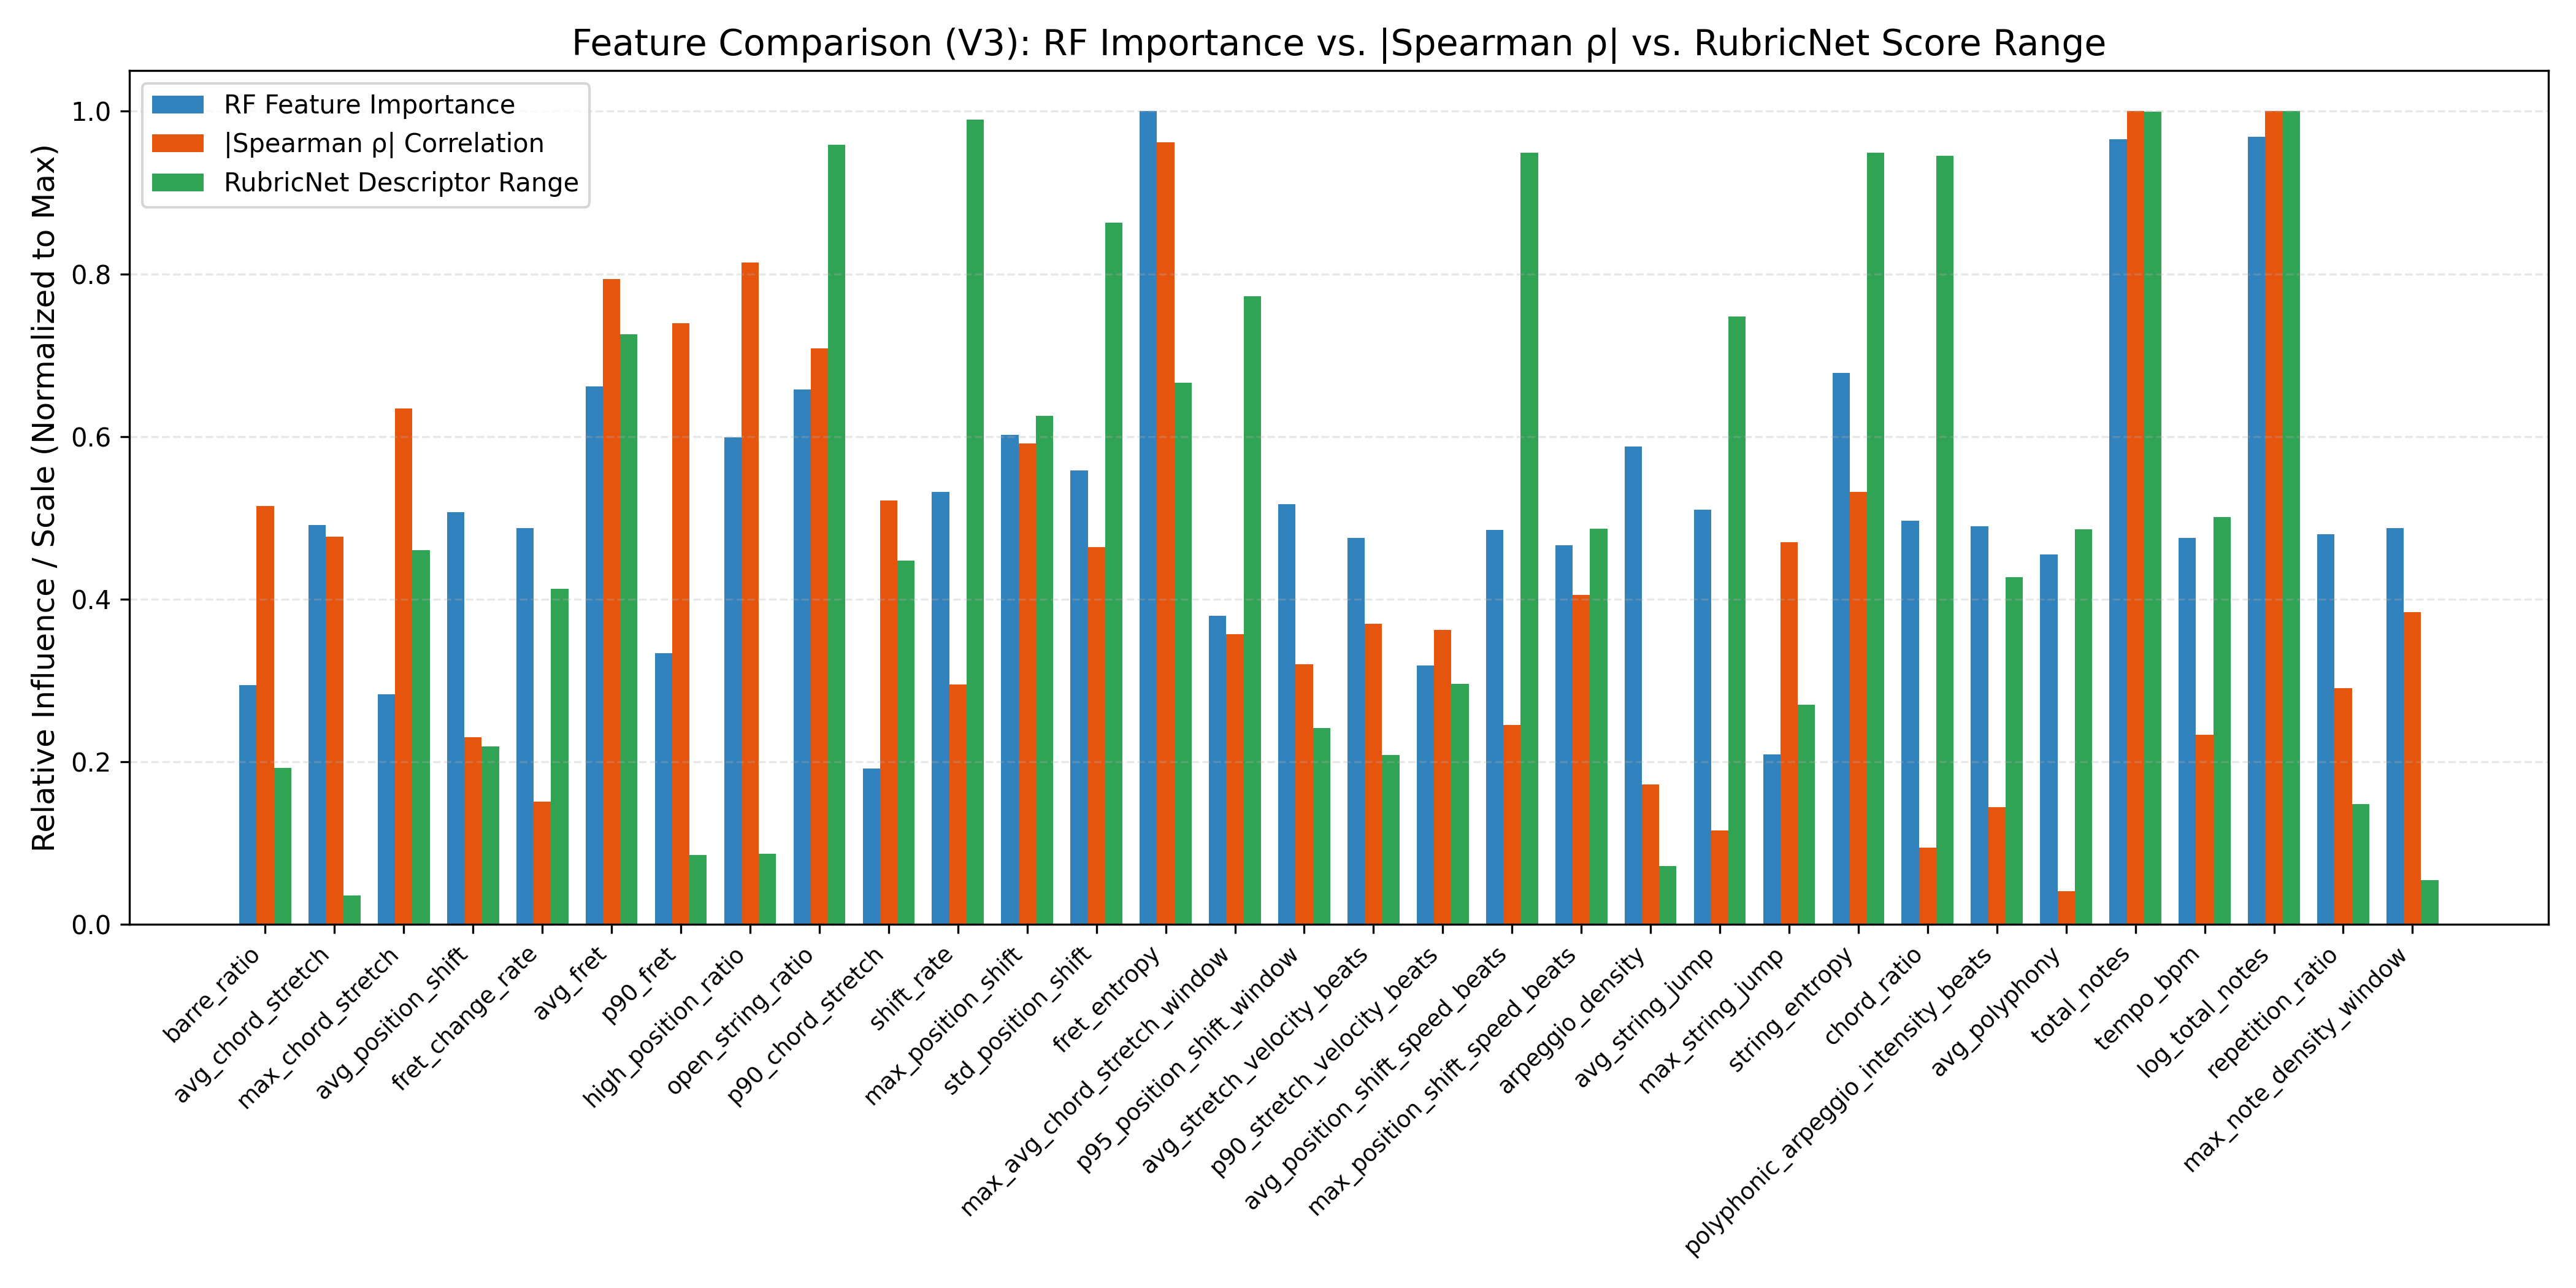
\includegraphics[width=\textwidth]{figures/importance_comparison_v3.png}
    \caption{Descriptor importance under three independent measures: RubricNet influence ranges, Random Forest feature importances, and absolute Spearman correlations with the raw difficulty labels (V3 descriptors, fold 0).}
    \label{fig:importance_comparison}
\end{figure}

A legitimate concern about any learned ``importance'' is that it may reflect training noise rather than signal. Figure~\ref{fig:importance_comparison} addresses this by triangulation: RubricNet's influence ranges are compared against two independent measures --- Random Forest feature importances and absolute Spearman correlations with the raw labels. The three paradigms broadly agree on which descriptors matter: \texttt{total\_notes}, the fret-coverage and position descriptors, and the movement statistics rank highly under all three, while the descriptors the audit flagged as weak remain near the bottom. The agreement across an additive neural model, an ensemble of trees, and a model-free rank statistic makes it unlikely that RubricNet's learned emphasis is an artifact of its own training.

\subsection{Monotonicity}
\label{sec:monotonicity}
For the rubric reading to be trustworthy, descriptor contributions should behave monotonically: pieces in higher difficulty classes should, on average, receive higher scores from difficulty-increasing descriptors. In an unconstrained network there is no reason for this to hold. In RubricNet, each $g_i$ is a monotone function of its input by construction (an affine map through tanh), but monotonicity \emph{across difficulty classes} is an empirical property of the data and training, not a guarantee.

\begin{figure}[htbp]
    \centering
    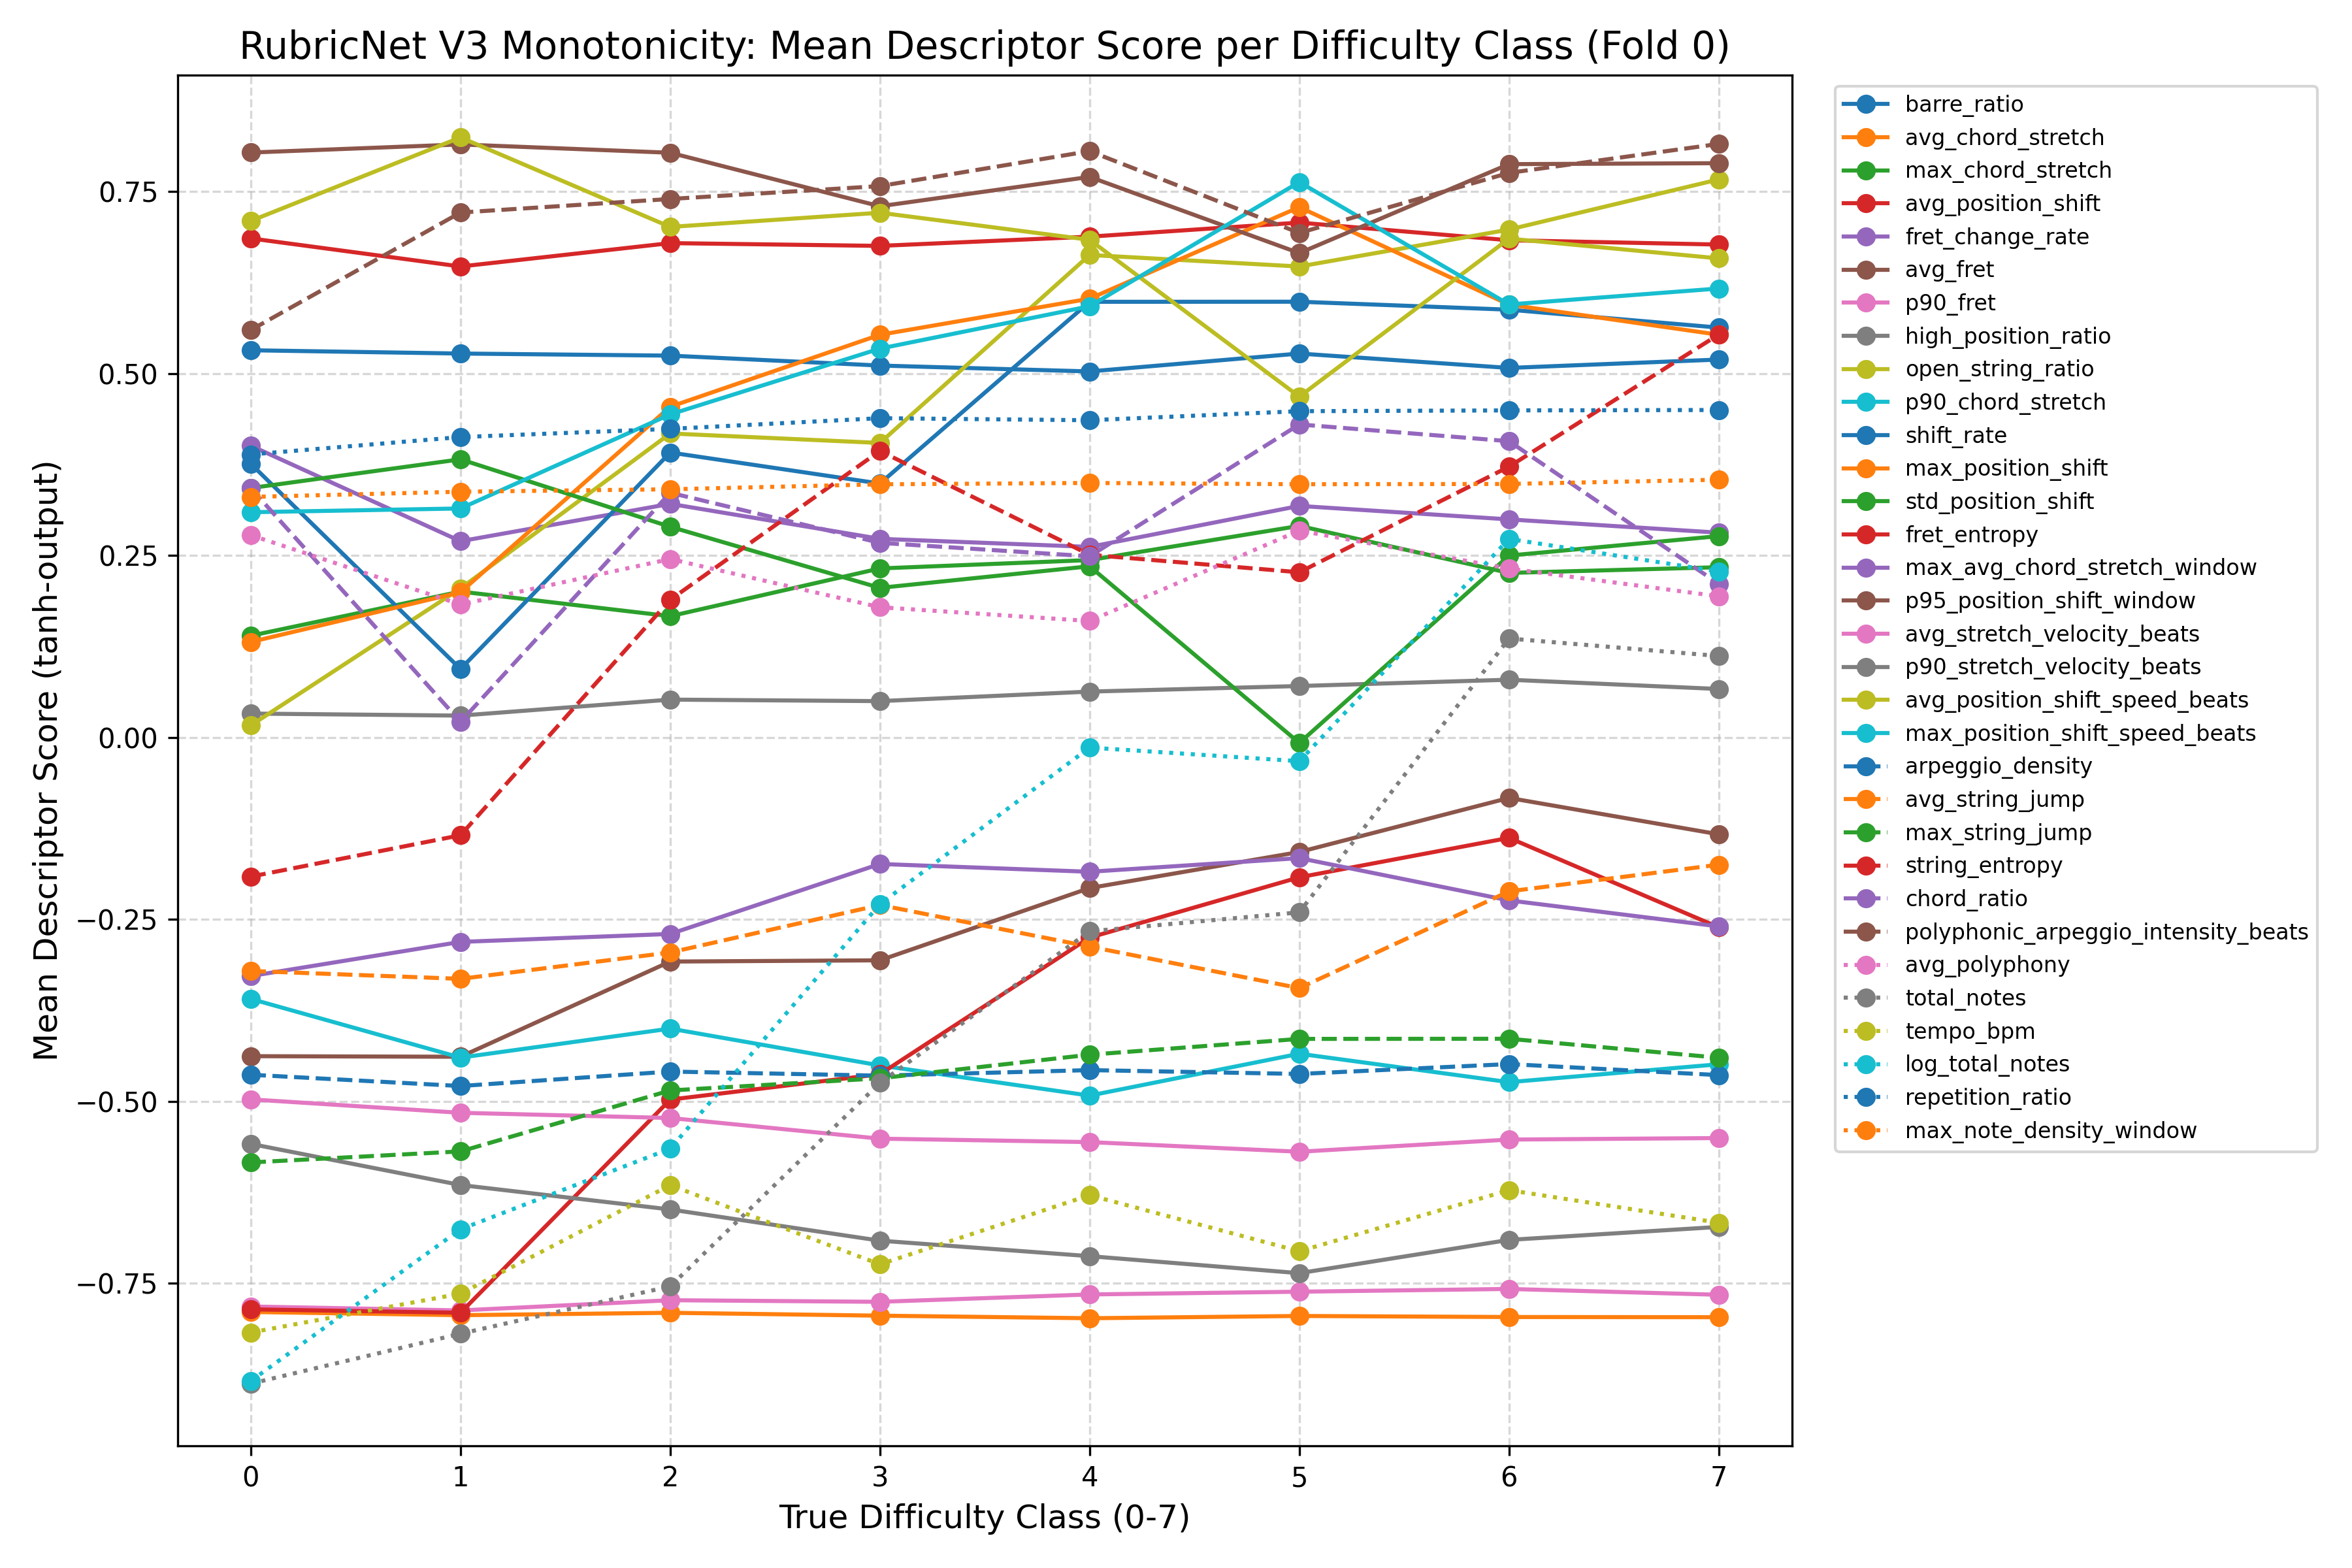
\includegraphics[width=\textwidth]{figures/monotonicity_v3.png}
    \caption{Mean per-descriptor subnetwork output by true difficulty class (V3 model, fold 0). Contributions rise steadily with difficulty for the influential descriptors; \texttt{open\_string\_ratio} falls, consistent with open strings making music easier to play.}
    \label{fig:monotonicity}
\end{figure}

Figure~\ref{fig:monotonicity} plots the mean subnetwork output per true difficulty class. The influential descriptors show steady trends from class 0 through class 7 --- rising for the difficulty-increasing descriptors, falling for \texttt{open\_string\_ratio} --- while the low-influence descriptors stay flat or fluctuate within a narrow band, consistent with their small learned ranges: they vary, but they barely move the sum. This is the property that makes the model's explanations usable in practice: if a piece is graded class 5 rather than class 3, the difference decomposes into specific descriptor contributions --- more frequent shifts, higher positions, denser texture --- each of which moves in a direction a teacher can verify against the score.

\subsection{Context-Free vs.\ Context-Aware Descriptors}
\label{sec:context_aware}
The V3 design rests on the hypothesis that physical difficulty depends on the time available to execute a demand. Table~\ref{tab:proxy_comparison} tests this hypothesis directly, comparing Spearman correlations with the raw 1--20 labels for context-free descriptors and their context-aware counterparts on the 639-piece rhythm subset.

\begin{table}[htbp]
\centering
\caption{Context-free descriptors vs.\ their rhythm-aware counterparts: Spearman $\rho$ against raw difficulty on the 639 pieces with rhythm data.}
\label{tab:proxy_comparison}
\begin{tabular}{llll}
\toprule
\textbf{Context-free} & $\rho$ & \textbf{Context-aware} & $\rho$ \\
\midrule
\texttt{avg\_chord\_stretch} & $+0.33$ & \texttt{avg\_stretch\_velocity\_beats} & $+0.40$ \\
 & & \texttt{max\_avg\_chord\_stretch\_window} & $+0.39$ \\
\midrule
\texttt{avg\_position\_shift} & $+0.13$ & \texttt{avg\_position\_shift\_speed\_beats} & $+0.30$ \\
 & & \texttt{max\_position\_shift\_speed\_beats} & $+0.44$ \\
 & & \texttt{p95\_position\_shift\_window} & $+0.37$ \\
\midrule
\texttt{arpeggio\_density} & $-0.14$ & \texttt{polyphonic\_arpeggio\_intensity\_beats} & $+0.22$ \\
\bottomrule
\end{tabular}
\end{table}

Every context-aware descriptor outperforms its context-free source, and the position-shift family shows the starkest gap: raw shift distance is nearly uninformative ($\rho = +0.13$), because a large shift with ample time is not difficult --- easy pieces abound with leisurely jumps between phrases. Dividing the same quantity by the inter-onset time in beats more than triples the correlation ($+0.44$ for the peak variant). The arpeggio case is the most instructive: \texttt{arpeggio\_density} on its own correlates \emph{negatively} with difficulty, since constant string crossing is characteristic of easy arpeggio studies; only when scaled by polyphony and note rate does the descriptor recover the intended signal, namely that crossing strings is demanding when it happens quickly and while multiple voices must be sustained. These comparisons confirm the design hypothesis and explain why the V3 generation helped the additive model in particular: the interaction between demand and available time is precisely what RubricNet cannot learn on its own.

\subsection{Fuzzy Rules as Difficulty Descriptions}
\label{sec:fuzzy_qualitative}
Section~\ref{sec:fuzzy_method} noted that the fuzzy classifiers trail RubricNet primarily because they ignore the ordinal class structure, not because their induced rules are uninformative. Table~\ref{tab:fuzzy_rules} shows this directly: the five most relevant complete-search rules for the easiest class (0) and the hardest class (7), taken from fold 0.

\begin{table}[htbp]
\centering
\caption{Top-5 complete-search rules by relevance (Equation~\ref{eq:fuzzy_relevance}) for the easiest and hardest difficulty classes, fold 0.}
\label{tab:fuzzy_rules}
\begin{tabular}{lcc}
\toprule
\textbf{Class 0 (easiest)} & \textbf{Relevance} & \\
\midrule
\texttt{fret\_entropy} is very low & 0.394 & \\
\texttt{p90\_fret} is low & 0.384 & \\
\texttt{max\_chord\_stretch} is low & 0.371 & \\
\texttt{avg\_fret} is very low & 0.365 & \\
\texttt{max\_position\_shift} is very low & 0.333 & \\
\midrule
\textbf{Class 7 (hardest)} & \textbf{Relevance} & \\
\midrule
\texttt{max\_position\_shift} is high & 0.394 & \\
\texttt{fret\_entropy} is very high & 0.371 & \\
\texttt{p90\_fret} is very high & 0.358 & \\
\texttt{p95\_position\_shift\_window} is high & 0.343 & \\
\texttt{total\_notes} is very high & 0.338 & \\
\bottomrule
\end{tabular}
\end{table}

The two rule sets are near mirror images: the easiest class is characterized by low fret positions, small stretches, and stable hand position, while the hardest class is characterized by their high-value counterparts plus sheer piece length. This mirrors the descriptor influence and monotonicity findings of Sections~\ref{sec:influence} and~\ref{sec:monotonicity}, obtained through an entirely different, non-neural method --- further triangulating that these descriptors carry genuine difficulty signal rather than an artifact of RubricNet's training.

The fuzzy pattern tree selected for class 7 in fold 0 ($d_{\max} = 3$) is
\begin{quote}
\texttt{OR(\\
\hphantom{xx}AVG(max\_position\_shift IS high, total\_notes IS very high),\\
\hphantom{xx}avg\_string\_jump IS moderate\\
)}
\end{quote}
which reads as: a piece is very likely class 7 if it combines frequent large position shifts with a high note count, \emph{or} if the right hand jumps between strings at a moderate rate. Across all 40 induced trees (five classes $\times$ 5 folds excluding classes with too few positive examples in some tail folds), 28 (70\%) contain at least one negated leaf, in clear contrast to Heerde et al., who found their evolutionary and pattern-tree rules never selected a negated operator~\cite{heerde2020comparing}. On this dataset, negation is evidently useful --- for instance, ``\texttt{total\_notes} is NOT low'' rules out the easiest pieces without committing to a specific higher value, which the ablation in Section~\ref{sec:auxiliary} confirms: disabling negated leaves lowers fuzzy pattern tree accuracy from 0.268 to 0.235 and Kendall's $\tau$ from 0.484 to 0.385.

\section{Auxiliary Experiments}
\label{sec:auxiliary}
Several further experiments were conducted after the main results were established. Most produced negative results; they are reported here because each one either justifies a design decision or marks off an unproductive direction.

\subsection{Direct 20-Level Classification}
\label{sec:raw20}
The most natural objection to the 8-class formulation is that GuitarBurst's native scale has 20 levels, raising the question of why those are not predicted directly. This was attempted, with considerable effort: training on the raw 1--20 targets initially failed to converge, and required monotonic initialization of the output layer (weights fixed at 1, biases stepping down by 0.5 per class) as well as disabling the inverse-frequency class weights --- which, with only 3--8 pieces at levels 17--20, otherwise inject substantial gradient variance --- before convergence was achieved at all. A dedicated 15-trial hyperparameter search improved validation accuracy from 0.168 to 0.303, but test accuracy still reached only 18.2\%, with an MAE of 2.07 on the 20-level scale and Kendall's $\tau$ of 0.43; even mapped down to the coarse 3-class view it achieved just 43.5\%, far below the 67.6\% of the 8-class model evaluated in the same way. The conclusion is that 716 pieces cannot support 20-way ordinal classification --- the extreme classes are simply too sparse --- and the 8-class binning of Section~\ref{sec:binning} is a necessity rather than a convenience.

\subsection{Pruning Weak Descriptors}
\label{sec:pruning}
The V2 audit had flagged six surviving descriptors as weak ($|\rho| \le 0.16$): \texttt{tempo\_bpm}, \texttt{arpeggio\_density}, \texttt{fret\_change\_rate}, \texttt{avg\_string\_jump}, \texttt{chord\_ratio}, and \texttt{avg\_polyphony}. Since an additive model sums in every input, removing them appeared to be an obvious improvement. It was not: training RubricNet on the pruned 26-descriptor set \emph{reduced} accuracy from 0.310 to 0.302, roughly doubled the fold-to-fold variance, and collapsed one fold to 0.196 accuracy. A plausible explanation is that the tuned regularization (dropout 0.20, weight decay 0.064) already suppresses uninformative subnetworks effectively, while the additional inputs act as mild stabilizers; it may also matter that the hyperparameters were tuned for 32 inputs and reused unchanged for 26. In either case, the full descriptor set was retained.

\subsection{Ordinal Label Smoothing}
\label{sec:smoothing}
Sweeping the smoothing temperature over $T \in \{0.15, 0.3, 0.6\}$ against the frozen V3 hyperparameters showed a small, consistent improvement at $T = 0.15$ (accuracy 0.312, balanced accuracy 0.294, no fold collapse), while $T \ge 0.3$ was flat to worse --- over-softening erodes the very boundary signal the ordinal loss requires. The improvement is within one standard deviation of the baseline, so it constitutes a direction rather than a result; the headline V3 numbers use the unsmoothed loss.

\subsection{Multi-Task Coarse Auxiliary Head}
A second output head predicting the 3-class grouping was trained jointly with the 8-class objective, sharing the aggregated score $S(x)$. All tested loss weightings underperformed the single-task baseline (accuracy 0.293--0.307 vs.\ 0.310), consistently rather than catastrophically. The diagnosis is structural: in a standard multi-task network, the auxiliary task regularizes a wide shared representation, but RubricNet's entire shared trunk is a single scalar. The two heads can only compete over how that one number is shaped, and the coarse class boundaries do not coincide with the fine-grained thresholds.

\subsection{Refined Left-Hand Descriptors (V4)}
A fourth descriptor iteration refined the left-hand feature definitions and barre detection. It performed slightly \emph{worse} than V3 across the board (accuracy 0.306, balanced accuracy 0.288, MAE 1.089), with identical coarse 3-class accuracy. Since it improved nothing while altering definitions that were already validated, V3 remains the final descriptor set, and V4 is noted here only for completeness.

\subsection{Rhythm Ablation and Interaction Descriptors}
\label{sec:interaction_features}
After the main V3 results were established, the question arose whether further improvements were possible within the additive architecture. Two complementary hypotheses were tested: first, that the V3 rhythm-aware features might be adding noise rather than signal; second, that hand-crafted interaction descriptors (products or composites of existing features) could encode multi-factor difficulty that a single descriptor cannot capture.

\subsubsection{Rhythm Ablation}
To isolate rhythm's contribution, V3 base descriptors were extracted without the six rhythm-aware features (\texttt{max\_avg\_chord\_stretch\_window}, \texttt{p95\_position\_shift\_window}, \texttt{max\_note\_density\_window}, \texttt{avg\_stretch\_velocity\_beats}, \texttt{avg\_position\_shift\_speed\_beats}, \texttt{polyphonic\_arpeggio\_intensity\_beats}), leaving 20 non-rhythm descriptors. The Random Forest reached 0.325 accuracy on this reduced set (essentially unchanged from V3's 0.331, within the margin of imputation variance), while RubricNet dropped to 0.301 from 0.310. This indicates that the rhythm features, while not decisive for the ensemble model, provide a modest but genuine signal contribution to RubricNet that the more flexible model can substitute for from other inputs.

\subsubsection{Hand-Crafted Interaction Descriptors}
Five composite descriptors were designed to capture multi-factor difficulty:
\begin{enumerate}
    \item \textbf{\texttt{barre\_difficulty\_tempo}}: $\texttt{barre\_ratio} \times (1.0 + \texttt{std\_position\_shift})$ --- barres are harder when positions are unstable.
    \item \textbf{\texttt{stretch\_under\_time\_pressure}}: $\texttt{p90\_chord\_stretch} / (\min \text{ inter-onset interval} + 0.1)$ --- large stretches are harder when little time is available.
    \item \textbf{\texttt{position\_shift\_entropy}}: $\texttt{std\_position\_shift} \times \texttt{string\_entropy}$ --- frequent shifts combined with string variety compound the left-hand demand.
    \item \textbf{\texttt{open\_string\_efficiency}}: $(1.0 - \texttt{open\_string\_ratio}) \times (\texttt{max\_position\_shift} + 1.0)$ --- pieces that avoid open strings while shifting positions are harder.
    \item \textbf{\texttt{arpeggio\_stretch\_coupling}}: $\texttt{arpeggio\_density} \times \texttt{avg\_chord\_stretch}$ (if arpeggio density $> 0.1$, else 0) --- arpeggios spanning wide stretches are demanding.
\end{enumerate}
Each descriptor had a univariate Spearman $|\rho|$ in the range 0.21--0.46 against the raw 1--20 difficulty labels, indicating meaningful individual signal. However, when appended to the V3 base feature set, all three model families suffered consistent degradation, as Table~\ref{tab:interaction_results} shows.

\begin{table}[htbp]
\centering
\caption{Effect of interaction descriptors: RubricNet, ordinal regression, and Random Forest all declined when interaction features were appended to the V3 base descriptors.}
\label{tab:interaction_results}
\begin{tabular}{lccc}
\toprule
\textbf{Model} & \textbf{Baseline (V3 Base)} & \textbf{+ Interactions} & \textbf{Change} \\
\midrule
RubricNet & 0.301 acc & 0.285 acc & $-$0.016 \\
Ordinal Regression & 0.325 acc & 0.282 acc & $-$0.043 \\
Random Forest & 0.325 acc & 0.310 acc & $-$0.015 \\
\bottomrule
\end{tabular}
\end{table}

The root cause is architectural. Each interaction descriptor is a product (or multiplicative composite) of features already present in the set. In an additive model, appending such derived features creates collinearity: the product does not contribute independent information, but reweights its parent features through the nonlinearity. The regularization (dropout and $\ell_2$ weight decay), tuned for the 20-descriptor base set, then struggles to suppress the noise in the new redundant dimensions, degrading generalization. Non-additive models can in principle exploit interactions through learned feature combinations; the strictly additive constraint prevents RubricNet from benefiting.

This experiment exposed a fundamental architectural limitation: \textbf{the additive model cannot be improved by appending collinear feature products}. Guitar difficulty does appear to depend on multi-factor interactions --- stretch difficulty depends on available execution time, for instance --- but capturing them within an additive setting requires either the hand-crafted context-aware descriptors already used in V3, which encode specific expected interactions without introducing collinearity, or relaxing the additive constraint at the cost of interpretability. Given that the central claim of this thesis rests on interpretability, V3 remains the final model. The implications are discussed further in Section~\ref{sec:disc_interpretability}.

\subsection{Fuzzy Rule Ablations}
\label{sec:fuzzy_ablation}
Three design choices behind the fuzzy classifiers of Section~\ref{sec:fuzzy_method} were tested against alternatives, each on the full 5-fold protocol.

\emph{Normalization.} Replacing the CDF-based fuzzification with plain min-max normalization slightly \emph{improved} both methods (complete search: accuracy 0.271, $\tau$ 0.557 vs.\ 0.264/0.464; fuzzy pattern tree: accuracy 0.278, $\tau$ 0.533 vs.\ 0.268/0.484). This is a mild surprise given the heavy-tailed descriptors motivating the CDF choice; a plausible explanation is that min-max preserves absolute magnitude differences between pieces that the CDF's rank-based mapping discards, and for a task with as few training pieces per fold as this one, that extra information outweighs the robustness benefit. The headline results nonetheless use the CDF variant, since it is the more faithful reading of evenly spaced linguistic terms on skewed features and the difference is within one standard deviation.

\emph{Balanced vs.\ plain RMSE.} Switching fuzzy pattern tree induction from class-balanced to plain RMSE left accuracy essentially unchanged (0.278 vs.\ 0.268) while leaving $\tau$ comparable (0.537 vs.\ 0.484); no fold produced a degenerate constant-output tree under either setting. The imbalance in this task (up to 3.7$\times$) is evidently mild enough that plain RMSE does not collapse to majority-class prediction here, unlike the more skewed one-vs-all splits anticipated in Section~\ref{sec:fuzzy_method}. The balanced variant is kept as the default since it carries no measurable cost and guards against the failure mode on splits where it would matter.

\emph{Negated leaves.} Disabling negation in fuzzy pattern tree induction is the one ablation with a clear, substantial effect: accuracy drops from 0.268 to 0.235, MAE rises from 1.469 to 1.754, and $\tau$ falls from 0.484 to 0.385. Unlike Heerde et al., who found negated operators were never selected in their genre-classification setting~\cite{heerde2020comparing}, 70\% of the trees induced here use at least one negated leaf (Section~\ref{sec:fuzzy_qualitative}). Negation is therefore not merely a faithfulness extension of the source paper but a genuinely useful addition on this dataset, and is kept enabled by default.
